\documentclass{article}

\usepackage[english]{babel}
\usepackage[a4paper,top=2cm,bottom=2cm,left=3cm,right=3cm,marginparwidth=1.75cm]{geometry}

\usepackage{amssymb}
\usepackage{amsfonts}
\usepackage{amsmath}
\usepackage{graphicx}
\usepackage{minted}
\usepackage{parskip}
\usepackage{pdflscape}
\usepackage{tcolorbox}
\usepackage{multicol}
\usepackage{tree-dvips}
\usepackage{qtree}

\usepackage[colorlinks=true, allcolors=blue]{hyperref}

\title{Solving 2048 with Expectimax}
\author{David Cook}

\begin{document}
\maketitle

\tableofcontents
\newpage
\begin{abstract}
The simplest goal of this project is to play the puzzle game 2048 with the expectimax algorithm. I intend to make it able to play any size of the 2048 game, though eventually, any algorithm will become impractical if the grid is too large. To mitigate this, I intend to find ways of pruning the tree as much as possible. Officially the game of 2048 ends when the tile of 2048 is achieved, the game can be continued until no more moves are possible.
A video of the program running can be found here \cite{video}.
\end{abstract}
\section{Introduction}
\label{sec:intro}
\subsection{The Problem}
\label{subsec:problem}
2048 is a game which features a 4x4 grid containing powers of 2. Each game starts with two cells, with a value of either 2 or 4.
All the tiles can be slid in any of the four directions (up, down, left and right); all the tiles can move simultaneously. When two of the same powers of 2 collide, the tiles merge, creating the next power of 2. The new tile increases the score by its new value. After each move, a new tile (either 2 or 4) will appear in a random free cell \cite{game2048}.

The goal of this project is to play a 2048 game using an AI-search algorithm. Some previous projects have reached the tile of 32k\cite{_16k2048ai}. Reaching 32k is uncommon; many expetimax implementations are only capable of reaching 4096 \cite{aiplays2048}\cite{expectimax2048}. 

A promising search algorithm is expectimax \cite{aiplays2048}. This is an algorithm designed for scenarios where there are two agents, one making random decisions and one making rational decisions \cite[~p.200]{russell2010artificial}. In some situations, it is possible to pre-compute a decision tree, saving execution time.
It is not practical to pre-compute a traditional 2048 decision tree, particularly when factoring in variable-size games.

Expetimax is also the algorithm used by \cite{_16k2048ai}, the implementation capable of reaching a tile of 32k, however, this is optimised to the point where the code is difficult to understand, for example the game's state appears to be stored a 64-bit unsigned integer, and modified using bitwise operations.

\subsection{Deliverables}
\label{subsec:deliverable}
\subsubsection{Proof of concept programs}
\begin{enumerate}
    \item Decision Tree
    \item Simple Expectimax Example
    \item 2x2 2048 Game
    \item 2048 with a heuristic
\end{enumerate}
\subsubsection{Report}
\begin{enumerate}
    \item Professional Issues: Licensing. (interim report)
    \item Design patterns in AI search. (interim report)
    \item Techniques used by humans and previous automated solvers. (interim report)
    \item User interface design for the solver. (interim report)
    \item Complexity and big $O$ notation. (interim report)
    \item NP Hardness
    \item The practicality and the effectiveness of the pruning expectimax tree.
    \item The heuristics have been generalised to support more 2048 games.
    \item Describe interesting algorithms and programming techniques, such as expectimax, used in the project.
    \item Implementation and performance of the decision tree.    
\end{enumerate}
The report will describe the implementation and optimisations of the expectimax algorithm, focusing on any software engineering principles used in the processes. 
\subsubsection{Final Program}
The final program will:
\begin{enumerate}
    \item Be written in java, with a full Object-oriented design, using modern software engineering principles.
    \item Be theoretically capable of playing any $n \times m$ 2048 game, though eventually break down due to performance.
    \item Have a user interface capable of keeping track of stats about the algorithms and an easy way of creating new $n \times m$ games.
\end{enumerate}
\newpage
\section{Proof of Concepts}
\label{sec:proof_of_concepts}
\subsection{Decision Tree}
\label{subsec:dt}
There are many ways of implementing a tree structure; various ones are more appropriate than others. The operations that are required in this situation are \cite{russell2010artificial}:
\begin{itemize}
    \item Generate a tree from the root node.
    \item Transverse the entire tree to calculate the score.
    \item Walk to a direct child node and regenerate the tree.
\end{itemize}
In the later case, the scores  will need to be regenerated on the pre-existing nodes and some new nodes node to generate.

I will assume generating a node can be done in $O(1)$ time; however, this may not be true. Generating or traversing nodes in a tree with $n$ nodes can not be done in $O(n)$ time. Reading a direct child can not be done in $O(1)$ time.

A common approach to making a tree is using a simple node class such as:
\begin{minted}{java}
public class Node {
    float score;
    Node[] children;
}
\end{minted}
This is a node with an array of references to its child nodes. Traversing this entire tree will have a time complexity of 
$O(n)$. Arranging these nodes into a tree structure takes $O(n)$ and finally picking a direct child of a node takes $O(1)$,
This simple implementation of a tree is adequate for the job, so more complex tree solutions are not necessary.

\subsection{Expectimax}
The expectiminimax algorithm allows for games to play with two rational agents and an element of chance \cite[p.~200]{russell2010artificial}. A simplified version of this algorithm, using only one rational agent, called expectimax, is able to perfectly model a game 2048. I intended to create an arbetry expectimax tree and calculate the scores of each node.
\label{subsec:expectimax}
\begin{figure}
    \centering
    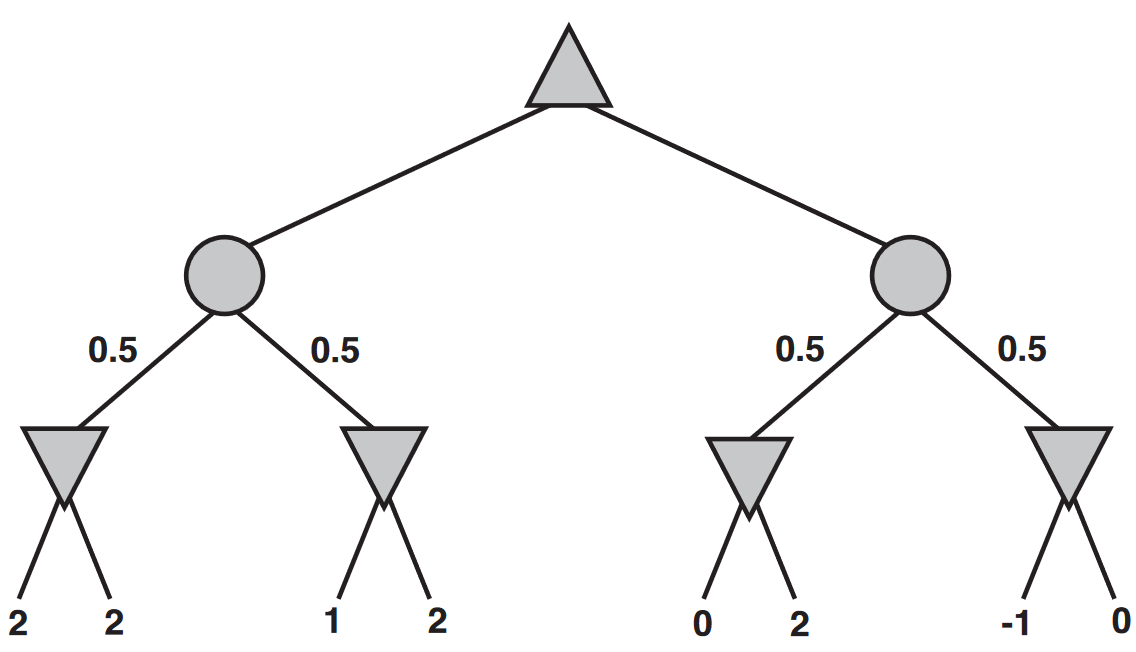
\includegraphics[width=0.7\textwidth]{expectimax.png}
    \caption{An expectiminimax tree example \cite[p.~200]{russell2010artificial}}
    \label{fig:expectree}
\end{figure}
The decision tree required in the expectiminimax algorithm (Figure \ref{fig:expectree}) has four types of nodes. However, three nodes are needed for the problem of solving 2048. These three types of nodes include:
\begin{itemize}
    \item Terminus nodes: These nodes are the leaves of the tree. Their score is already known and used to calculate the score in the rest of the tree.
     \item Chance nodes: These nodes represent situations where there are random states that may follow. The weights between
    a chance node and its children represent the probability of that event occurring. A chance node's score is the weighted sum of its children.
    \item Maximising nodes: These nodes take the score of the maximum-scoring child.
    \item Minimising nodes: These nodes take the score of the minimum-scoring child.
\end{itemize}
Each of these three relevant types of nodes has been converted to individual java classes, caching the scores in a float
attribute, so they only need to be calculated once.

Figure \ref{fig:expectree} has 

\subsection{2048}
\label{subsec:2048}
This proof of concept was created mostly using one source \cite{source2048}, the original 2048 source code. While I did not
directly copy any of the code, I read through most of the code relevant to the key features of the game and tried to understand 
why things were done that way. I then re-wrote the code in java using similar approaches.

I learnt a few things that were very useful while writing this prototype. For example: 
\begin{itemize}
    \item If you loop over the numbers in the wrong order, a tile may collide with a tile that will be moved later. 
    See Figure \ref{fig:slidebug} for an example.
    \begin{figure}
        \centering
        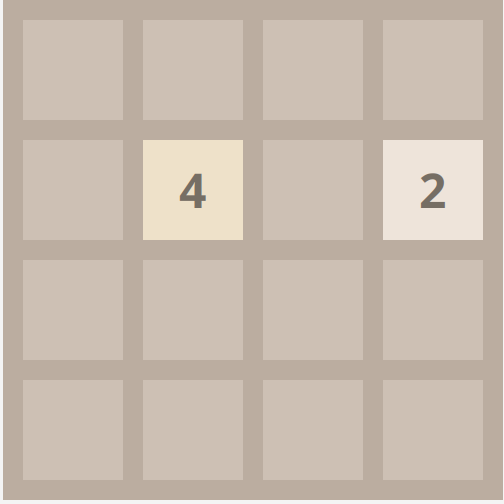
\includegraphics[width=0.3\textwidth]{2048_slide.png}
        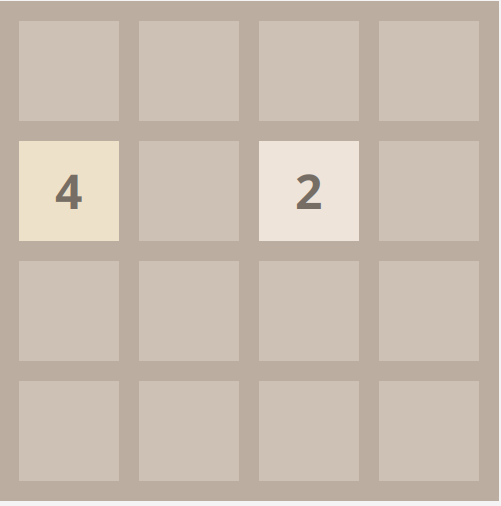
\includegraphics[width=0.3\textwidth]{2048_slide2.png}
        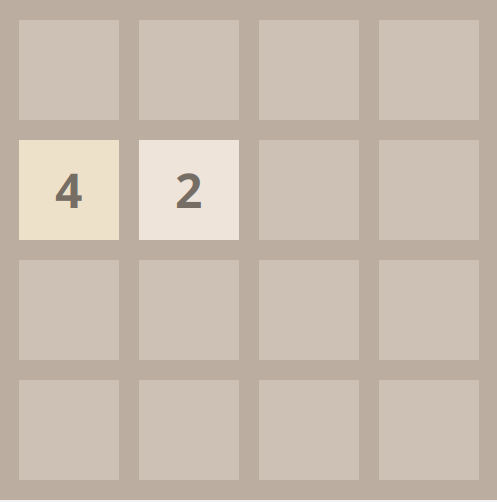
\includegraphics[width=0.3\textwidth]{2048_slide3.png}
        \caption{The first image shows a state shown before a left slide, the second one shows after an incorrect left slide, and the third one shows after a correct left slide.}
        \label{fig:slidebug}
    \end{figure}
    \item When merging tiles, you need to ensure that you do not merge a tile multiple times. See Figure \ref{fig:mergebug} for an example.
    \begin{figure}
        \centering
        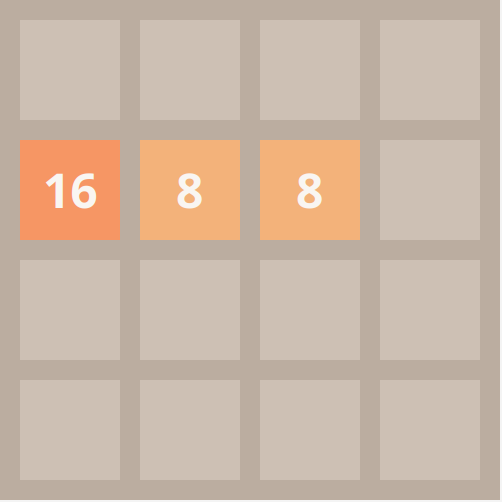
\includegraphics[width=0.3\textwidth]{2048_merge.png}
        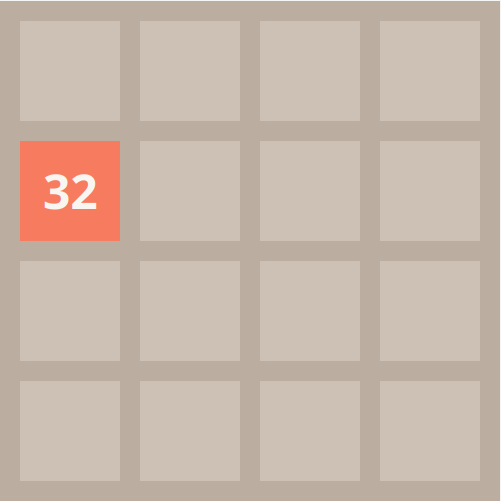
\includegraphics[width=0.3\textwidth]{2048_merge3.png}
        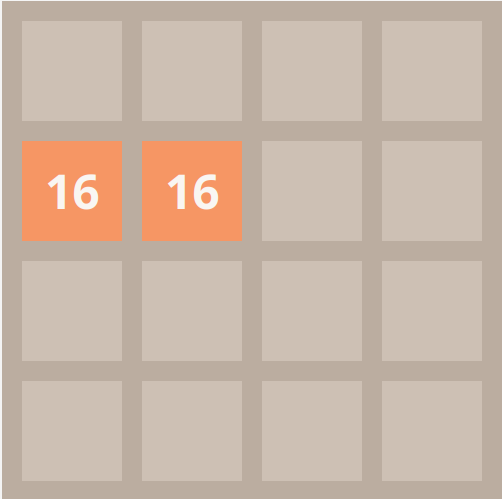
\includegraphics[width=0.3\textwidth]{2048_merge2.png}
        \caption{The first image shows a state shown before a left slide, the second one shows after an incorrect left slide, and the third one shows after a correct left slide.}
        \label{fig:mergebug}
    \end{figure}
\end{itemize}
My test suite picked up the first issue; however, I had not considered the second case before writing the proof of concept. I only caught the second issue because I wrote a command line user interface (see figure \ref{fig:2048_cli} allowing me to play the game and pick up on bugs). 

    \begin{figure}
        \centering
        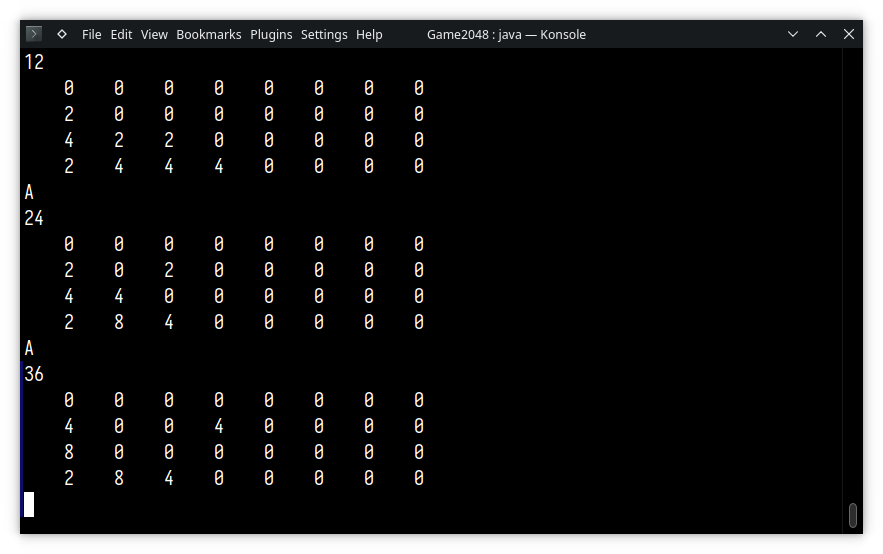
\includegraphics[width=0.8\textwidth]{Screenshot_20221201_231121.png}
        \caption{Command line user interface used by 2048 prototype playing a 4 x 8 game.}
        \label{fig:2048_cli}
    \end{figure}
\subsection{2048 with Expectimax}
\label{subsec:2048_expectimax}
A working prototype of expectimax has been developed (see \ref{subsec:expectimax}). A working 2048 prototype has also already been developed as well (see \ref{subsec:2048}).  These components need to be modified so that the expectimax algorithm can be applied to 2048 game. 
The aim is to generate the full tree instead of using a heuristic but to do this; the 2048 puzzle must be simplified.

Two modifications were made to the setup of 2048 to ensure the tree was a reasonable size:
\begin{itemize}
    \item Make the game $2 \times 2$.
    \item After a move, only the number 2 can appear.
\end{itemize}
With these modifications, there are at most only three possible free cells where a tile can be added. With possible moves, the tree can only grow by $3 \times 4 = 12$ for each move.
A traditional 2048 game has four possible moves and 15 possible free cells where a tile can be added, meaning the tree can grow by $15 \times 4 = 60$ for each move.

Originally the only modification to the game was making it $2 \times 2$ to increase the tree by $6 \times 4 = 24$ for each move. However, the prototype could not calculate the tree within a reasonable time. Hence why the new tiles are limited to just the '2' tile to reduce the complexity further.
\subsection{Heuristic for 2048}
\label{subsec:heuristic}
In this prototype, the restrictions were removed from the game. The size of the game is now $n \times m$, and either a $2$ or $4$ can appear in the grid. This makes it impracticable to calculate the full tree. To do this, an arbitrary  %depth% limit is chosen for the tree. At the leaf nodes in the tree, a heuristic value is calculated. 

Two different heuristic functions were implemented.
\begin{itemize}
    \item Sum up all the items in the grid. This was a simple heuristic to ensure that the algorithm worked as expected. This heuristic could not achieve high scores.
    \item Sum up all the values multiplied by the row they are in (Top row = 1 and bottom row = n). The most rewarding path was placing larger numbers lower in the grid.  This heuristic was much more effective, reaching a tile of 512.
\end{itemize}

With this, the algorithm can theoretically be applied to any 2048 game, which becomes impractical for a large $depth, n$ or $m$. The original plan was to apply this to a 2x2 game; however, due to the nature of the heuristics, I removed this requirement and allowed any size of the grid, as the $depth$ limit makes this practical.
\section{User Interface Design}
\label{sec:ui}

The user interfaces resemble the original 2048 game, as shown in Figure \ref{fig:2048interface}.
Parts of the user interface are appropriate for my solver. However, some features must be removed.

\begin{figure}
    \centering
    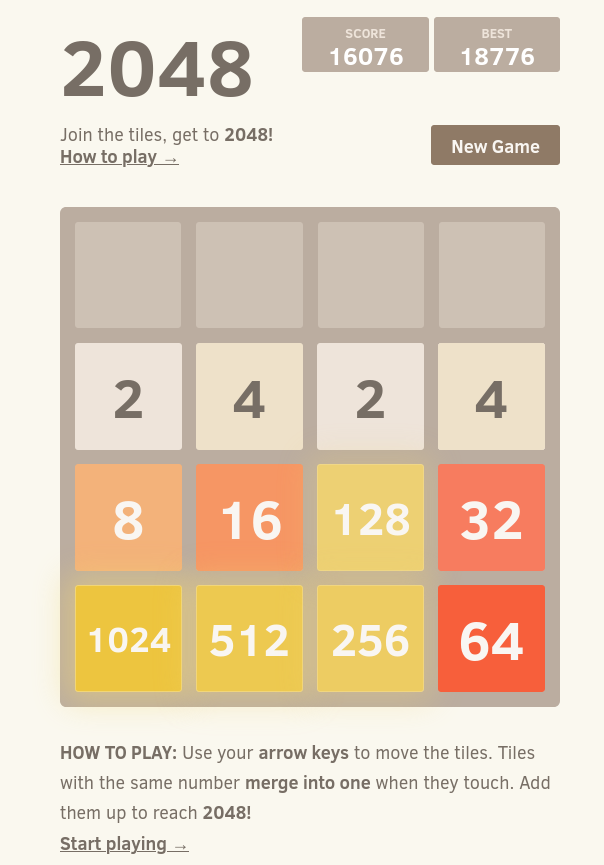
\includegraphics[width=0.4\textwidth]{2048-interface.png}
    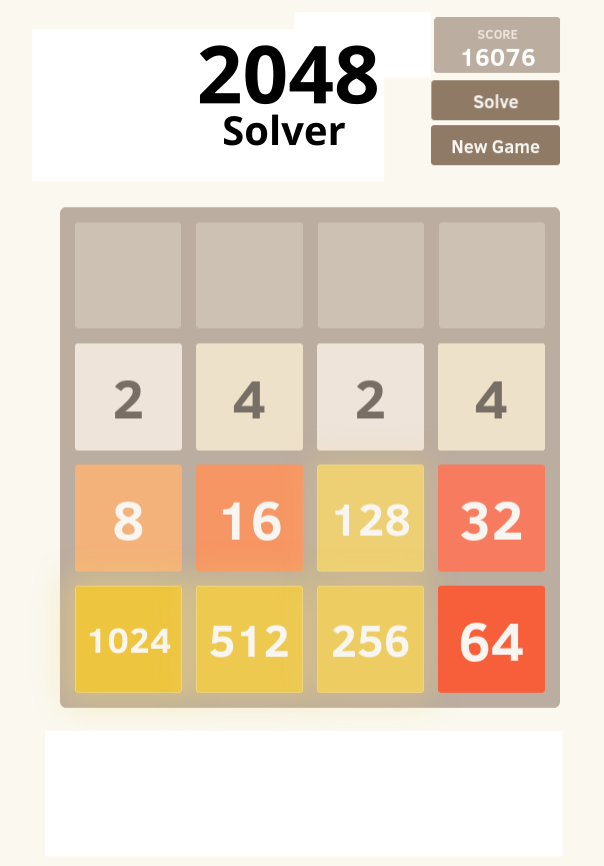
\includegraphics[width=0.4\textwidth]{interface-mockup.png}
    \caption{On the left is a screenshot of the official 2048 user interface \cite{game2048} and on the right
    is an edited version of this image designed to represent what my main interface might look like}
    \label{fig:2048interface}
\end{figure}

Firstly the instructions on how to play the game seen at both the top and bottom of the page have been removed
as the game will play itself. Secondly, a new solve button has been added.

The 'best' score box has been removed from the interface. I will need to keep track of more data than the best score to evaluate how effective the algorithm is and will likely log this in a CSV file.

Most versions of 2048 have an animation that plays as the tiles slide; while this would be possible, as animations do exist in JavaFX \cite{javadocfx}, I am not familiar with them and think it is not worth the time to re-implementing the animations.

When creating a new game, it is important that the user can enter the size of the new game; however, this input should not be visible when the user doesn't want to make a new game. A long-established solution is providing the user with a popup dialogue asking for the size of the game. There is no reference for this in the original 2048 to base the user interface on, so instead of modelling an existing interface, I have created a mock-up of what the interface should look like figure \ref{fig:popup}

\begin{figure}
    \centering
    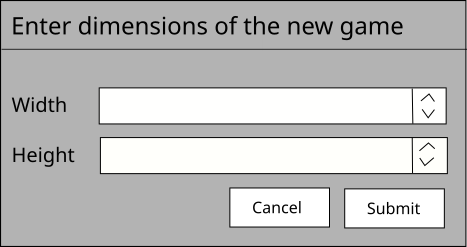
\includegraphics[width=0.4\textwidth]{newGamePopup.png}
    \caption{Mock up of the new game popup window.}
    \label{fig:popup}
\end{figure}
\section{Design Patterns for AI Search}
\label{sec:dp}
There are many ways design patterns can be used in AI search algorithms, specifically in the expectimax algorithm. Figure \ref{fig:alg_uml} shows the structure of the code used for the algorithm; there are a few changes that have been made that have not yet been implemented.


\subsection{Factory Design Pattern}
\label{subsec:factory}
A factory design pattern is a creational design pattern used to hide the complexity of creating an instance of a class \cite{CS2800_creational}. This implementation of the expectimax algorithm includes three types of nodes:
\begin{itemize}
    \item \mintinline{java}{MaxNode}
    \item \mintinline{java}{ChanceNode}
    \item \mintinline{java}{LeafNode}
\end{itemize}
The  expectimax tree will always start with a maximising node. This means that despite the complexity of the Node classes, given a game state and the maximum depth of the tree, it is very simple to create the root node of the initial tree. Generating the child nodes is slightly more complex than the initial root node. Depending on the parent and if the node has children, it can be any of the three node types. For this, two creational methods can be created. One is to create an initial root node that only takes in a small amount of information and one that is package private that takes in more data to determine what type of node it is.
\subsection{Singleton Design Pattern}
\label{subsec:singleton}
A singleton is a creational design pattern that ensures at most one class instance; if an object is required multiple times, the same object is returned each time \cite{CS2800_creational}.

The most clear-cut case for this design pattern is the heuristic classes. The existing heuristic classes have no attributes, just two methods. This means that if multiple class instances were created, they would
always be equivalent. This means there is no benefit from having multiple objects for these; a Singleton design pattern is a logical choice.

Another case where a singleton pattern could be used is for the Node Factory. Currently, this is just a class containing only static methods. The only situation where two different instances of this factory would be useful is playing multiple 2048 games simultaneously with different random number generators, which seems unlikely.
\subsection{Observer Design Pattern}
\label{subsec:observer}
An observer is a behavioural design pattern that is particularly useful when something needs to happen in an object based on an event in another object.
A common example of where this design pattern can be used is event handlers in a user interface \cite{CS2800_behavioural}.

An observer interface consists of one function, often called \mintinline{java}{notify()}, or \mintinline{java}{update()}. This function is called by an observable object when some event occurs.

In this project, there is a class called \mintinline{java}{Solver}, which contains the code for the expectimax algorithm. Each time it calculates, and makes, a move, this needs to be updated in the View. To make
this happen, an observer design pattern is used. Each time the observer is notified, it includes a parameter that describes the current state of the game, which is passed to the view to be displayed.
\subsection{Visitor Design Pattern}
\label{subsec:visitor}
Allows some processing to be done externally from the object (A). A second object (B) can visit object A, which accepts object B and finally runs the process on object A.  This is particularly useful when there are multiple ways something can be evaluated or multiple things to be evaluated \cite{CS2800_behavioural}.

To be practical, the expectimax algorithm applied to 2048 requires a heuristic function. There are many different heuristic functions, and there may be various reasons to use one over another in certain scenarios; it is convenient to separate the heuristic code from the \mintinline{java}{GameState} and apply the correct heuristic function when needed.

\begin{landscape}
\begin{figure}
    \centering
    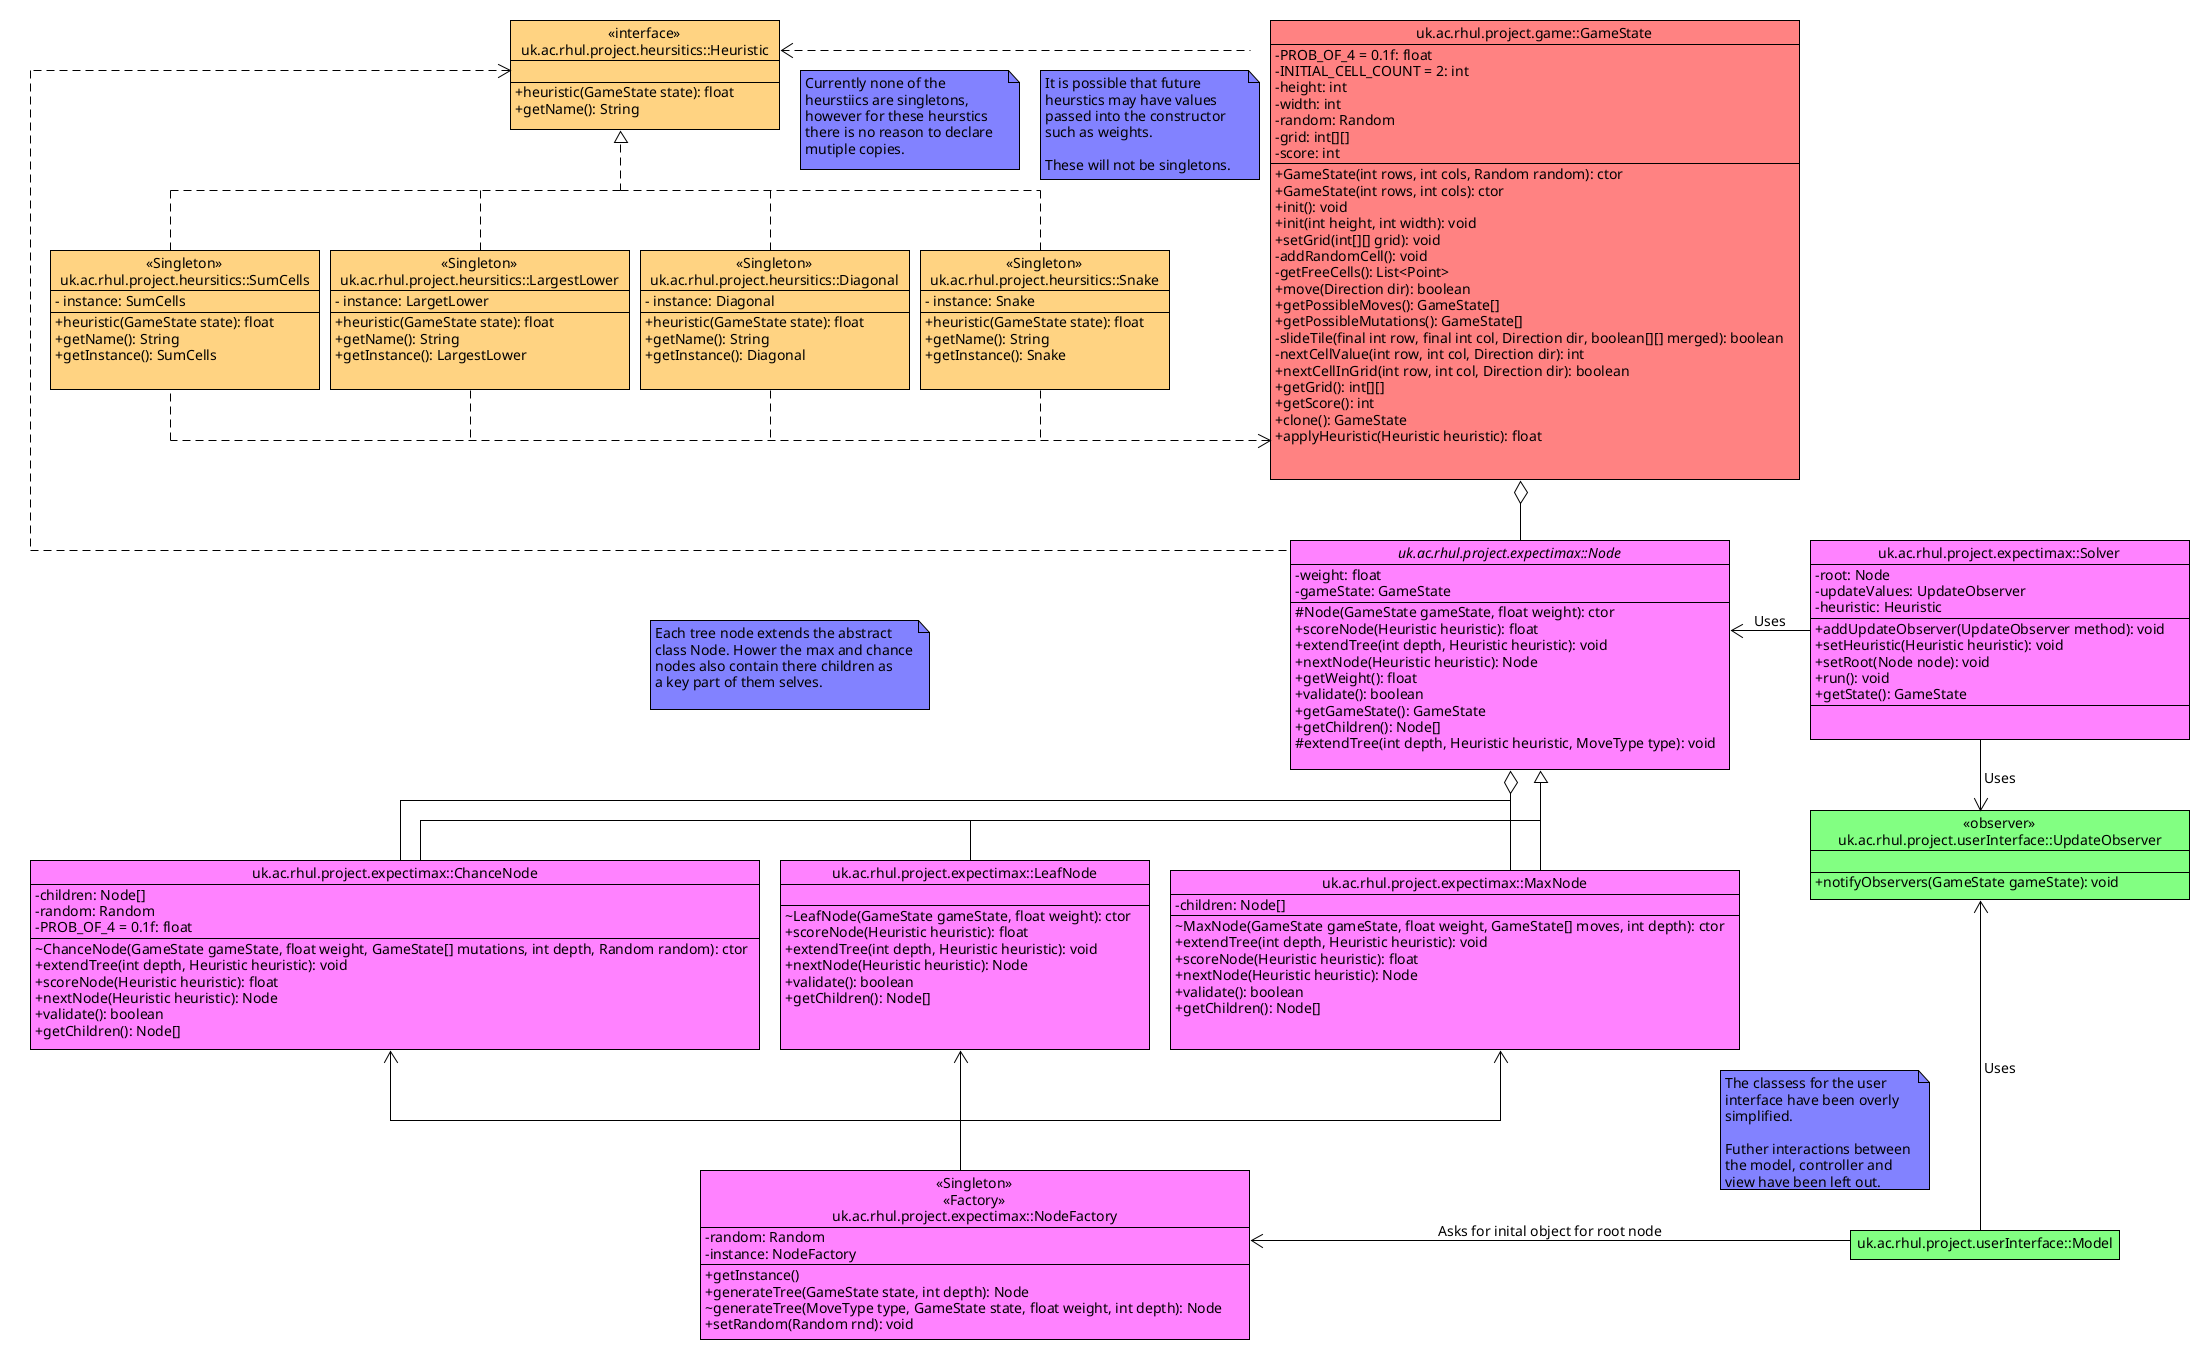
\includegraphics[width=1.5\textwidth]{algorithm_uml.png}
    \caption{UML Diagram representing the parts of the code related to the expectimax algorithm.}
    \label{fig:alg_uml}
\end{figure}
\end{landscape}
\section{Techniques used to solve the game}
\label{sec:techniques}

\subsection{Human Approaches}
\label{subsec:human_techniques}
It can be difficult to automate a human strategy however it is possible to reward or penalise certain states, and human strategies can be a good place to start when looking for features to reward or penalise.

One human strategy is to keep the largest number in a corner and have a gradient leading to the smaller values like in figure \ref{fig:gradient} \cite{strategy2048}. In testing, this way of arranging the grid makes it relatively easy to merge multiple tiles in a few moves and reduces the risk of trapped values. However, it does lead to many duplicate values that are difficult to merge, so there is often insufficient space to reach the larger tiles.

\begin{figure}[!tbp]
    \centering
    \begin{minipage}[b]{0.45\textwidth}
        \centering
        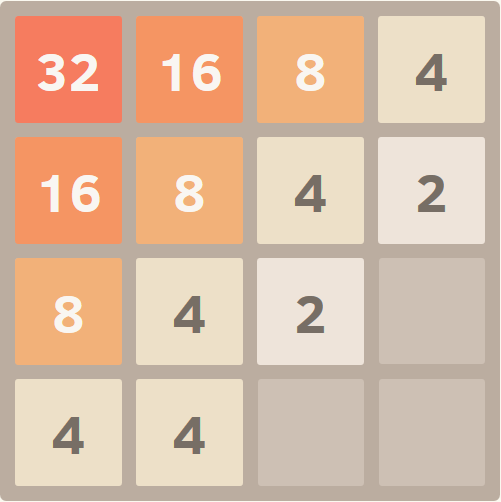
\includegraphics[width=0.5\textwidth]{gradient.png}
        \caption{Gradient pattern used in a 2048 human strategy \cite{strategy2048}.}
        \label{fig:gradient}
    \end{minipage}
    \hfill
    \begin{minipage}[b]{0.45\textwidth}
        \centering
        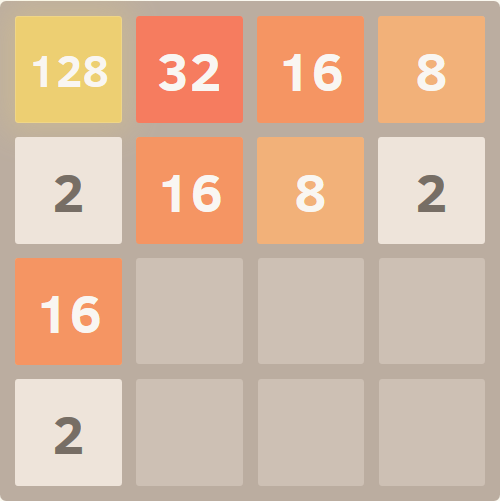
\includegraphics[width=0.5\textwidth]{trapped.png}
        \caption{Example of a trapped value in 2048 \cite{strategy2048}.}
        \label{fig:trap}
    \end{minipage}
\end{figure}
A trapped value is surrounded by larger numbers \cite{strategy2048}, such as the 2 in figure \ref{fig:trap}. Partially when there are not very many free cells around, these cells can be very difficult to get rid of and can take up useful space. They often appear when an empty tile is created after a merge in an area with large numbers. 

\begin{figure}
    \centering
    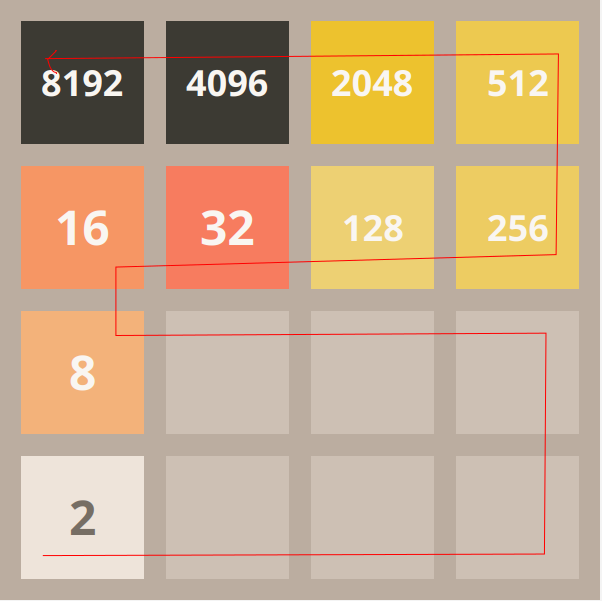
\includegraphics[width=0.2\textwidth]{bitmap.png}
    \caption{Snake pattern.}
    \label{fig:snake}
\end{figure}

Another approach is to try and order the tiles into ascending order using a snake shape (Figure \ref{fig:snake} \cite{aiplays2048}. The source for this approach describes an automated method; however,
humans can also use this. In testing, this was found to be a very reliable strategy, even reaching tile 8192. The main drawback of this approach was that when merging the row with the largest numbers, there is a risk of producing a trapped value. With careful planning and some luck, it is possible to recover from these states.
\subsection{Automated Approaches}
\label{subsec:automated_techniques}
Many algorithms can be used to solve 2048, to varying degrees of success. Some of these algorithms are \cite{approches2048}:
\begin{itemize}
    \item Minimax - assumes that two rational agents always make their most optimal move \cite{minmaxCS2910}, this strategy does not adapt very well to 2048, according to \cite{approches2048} when citing \cite{minmax2048}.
    \item Expectimax - This is a much more effective strategy, similar to Minimax; however, the second agent is assumed to make random decisions \cite[p.~200]{russell2010artificial}. This model lends itself much better to 2048 as it exactly matches what happens \cite{expectimax2048}.
    \item Monte-Carlo Tree-Search - "Produces asymmetric trees, effectively pruning poor paths allowing for deeper searching on paths with greater potential." \cite{approches2048}. This method was highly effective compared to Mini-max and Expectimax.
    \item Average Depth-Limited Search - "ADLS approximates expectimax by running multiple simulations; it does not try to calculate all possibilities. Instead, likely outcomes will repeat more often." \cite {approches2048}. This method was highly effective.
\end{itemize}
While there are many different algorithms, some can be very effective; this report will focus on the expectimax algorithm. This is a relatively simple but effective algorithm \cite{expectimax2048}. As discussed in section \ref{subsec:2048_expectimax}, calculating an expectimax tree for even a small 2048 game is normally impractical; for a traditional 2048 game, there are even more possibilities, leading to an even bigger complete expectimax tree. Previous projects have used a depth-limited expectimax tree \cite{aiplays2048}, sometimes even with a dynamic depth \cite{expectimax2048}.

A heuristic function is needed to evaluate how good a state is at the end of the tree. Two interesting heuristics will be covered in this section. 

\subsubsection{Snake Heuristic}
\label{subsec:snake}
The snake heuristic is based on the most effective heuristic in \cite{aiplays2048}.

This heuristic works by calculating a weighted sum of the values in the grid:
\[
    \text{Let }S\text{ be the state of the game, }W=\begin{bmatrix}
    4^{15}&4^{14}&4^{13}&4^{12}\\
    4^8&4^9&4^{10}&4^{11}\\
    4^7&4^6&4^5&4^4\\
    4^0&4^1&4^2&4^3
    \end{bmatrix} \]\[\text{and }h(S)\text{ be the heuristic function.}
\]\[
    h_1(S)=\sum_{i=1}^{4}\sum_{j=1}^{4}W_{i j}S_{i j}
\]

This heuristic takes the human strategy of organising into snake shape rewards boards where this strategy has been applied.
\subsubsection{Diagonal Heuristic}
\label{subsubsec:diag}
The diagonal heuristic is used in the project \cite{expectimax2048}.
Similar to the snake heuristic, part of this is a weighted sum. However, there is also a penalty.

The penalty function $p(i, j) = \sum |\text{difference between each nonzero neighbour}|$. 
For example, with the grid state:
\[
\begin{bmatrix}
128 & 64 & 32 & 16 \\
8 & 32 & - &- \\
32 & 16 &8 &-
\end{bmatrix}\]\[
P(2, 2) = |32 - 64| + |32 - 16| + |32 - 8| = 32 + 16  + 24 = 72
\]

The heuristic function, where $S$ is the games state, and
$
W=\begin{bmatrix}
    6&5&4&1\\
    5&4&1&0\\
    4&1&0&-1\\
    1&0&-1& -2\\
\end{bmatrix}
$ is:
\[
    h_2(S)=\sum_{i=1}^{4}\sum_{j=1}^{4}W_{ij}S_{ij}^2 - \sum_{i=1}^{4}\sum_{j=1}^{4}p(i,j)
\]
\begin{figure}
    \centering
    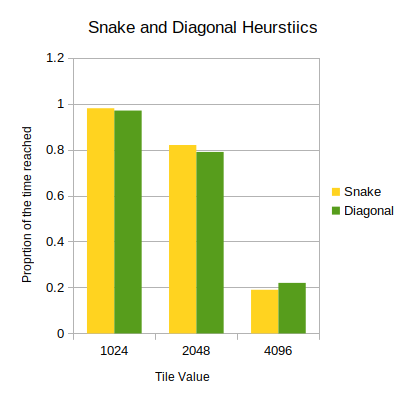
\includegraphics[width=0.4\textwidth]{SnakeToDiagonal.png}
    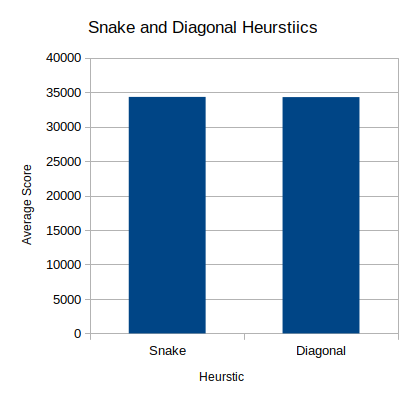
\includegraphics[width=0.4\textwidth]{SnakeToDiagonalScore.png}
    \caption{A compassion between the snake and the diagonal heuristics.}
    \label{fig:SnakeVDiagonal}
\end{figure}
\subsubsection{Compassion between Snake and Diagonal Heuristics}
After implementing these heuristics, the maximum tiles and scores were logged for 100 games using each heuristic. There was no statistically significant difference between the two heuristics, as shown in Figure \ref{fig:SnakeVDiagonal}. 



\subsection{Potential future heuristics}
During the second term, I would like to try applying the penalty, defined in section \ref{subsec:diag} function, to the snake heuristic multiplied by various weights.

Combing the snake and diagonal heuristic. Placing large numbers along one edge is a common strategy in 2048; however, the diagonal heuristic was very effective and quickly got mid range numbers; using the diagonal heuristic to get a mid-range number, such as 128 or 256,  but using the snake heuristic on the number tile at the same time.
For example, if the game state is.
\[
\begin{bmatrix}
    2048 & 512 & 128 & 16 \\
    - & 4 & 16 & 8 \\
    - & -  & 4 & - \\
    - & - & - & - \\
\end{bmatrix}
\]
The weights matrix may look something like this:
\[
\begin{bmatrix}
     7 & 6 & 5 & 4 \\
     2 & 3 & 4 & 3 \\
     1 & 2 & 3 & 2 \\
     0 & 1 & 2 & 1 \\
\end{bmatrix}
\]
\section{Time Complexity}
\label{sec:complexity}
\subsection{Complexity}
\label{subsec:time_comp}
\subsubsection{4 x 4 Game}
As the most effective heuristics are currently locked into a $4\times4$ game, I will calculate the time complexity when run on a $4 \times 4$ game, where $n$ is the maximum depth of the tree.

After each maximising node, the tree grows by at most 4. One for each possible move up, down, left and right.

A game starts with two cells; hypothetically, let's say:

\[
\begin{bmatrix}
    2&2&-&-\\
    -&-&-&-\\
    -&-&-&-\\
    -&-&-&-\\
\end{bmatrix}
\]
The best case outcome is that these two cells are merged:
\[
\begin{bmatrix}
    4&-&-&-\\
    -&-&-&-\\
    -&-&-&-\\
    -&-&-&-\\
\end{bmatrix}
\]
This leaves 15 free cells for the new cell to appear; after this, there will be two cells again.
Therefore there can never be more than $15$ free cells.

Therefore the most children a chance node can have is $15\times2=30$.



Each node has constant time work, so the leaf nodes dominate the tree.



For every two layers, the number of leaf nodes multiplies at most $120$, and there are $n$ layers in the tree. Therefore their are $120^\frac n 2$ leaf nodes
$\therefore$ time complexity to calculate the next move is $120^\frac n 2 = O(\sqrt{120}^n) \approx O(10.954^n)$

\subsubsection{m x n Game}
Consider calculating the children of a max node: each max node has at most 4 children, and each child's state is calculated using the following code (see uk.ac.rhul.project.game.GameState):
\begin{minted}{java}
boolean move(Direction dir)
{
    ...
    for (int i : dir.getVerticalStream(this.height))
    {
        for (int j: dir.getHorizontalStream(this.width))
        {
            if (grid[i][j] != 0 && this.slideTile(i, j, dir, merged)) ...
        }
    }
    return flag;
}

private boolean slideTile(final int row, final int col, Direction dir, boolean[][] merged)
{
    int target_row = row;
    int target_col = col;

    // Calculate how far the tile can be moved (assuming no merge)
    while (nextCellInGrid(target_row, target_col, dir) && this.nextCellValue(target_row, target_col, dir) == 0)
    {
        target_row += dir.getRows();
        target_col += dir.getCols();
    }

    ...
}
\end{minted}

$\Rightarrow$ For directions UP and DOWN, the time complexity of the move operation is $O(m^2n)$ and for LEFT and RIGHT the time complexity is $O(mn^2)$

$\Rightarrow$ calculating the children of the max node has time complexity $2O(mn^2) + 2O(m^2n)$.

Consider calculating the children of a chance node:

A grid has at least one nonzero tile $\therefore$ There are $mn - 1$ cases to consider.

\begin{figure}
    \centering
    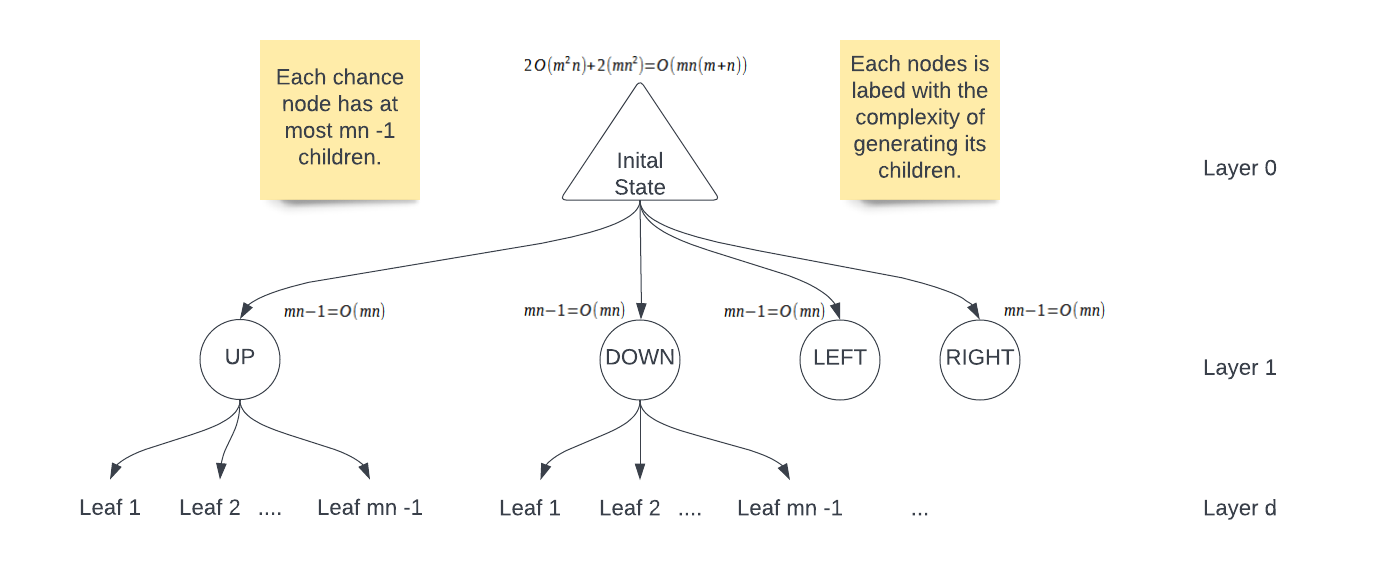
\includegraphics[width=0.8\textwidth]{expectimax tree.png}
    \caption{A tree for a $n \time m$ 2048 game}
    \label{fig:nm2048}
\end{figure}

By looking at Figure \ref{fig:nm2048}, it can be deduced that the number of work increases after every pair of layers, and the amount of work done generate the last two layers $d - 1$ and $d$ is: 

\begin{align}
\text{Time Complexity} & = 4^\frac{d}{2}(mn - 1)^{\frac{d - 2}{2}}O(mn(m+n)) + 4^\frac{d}{2}(mn - 1)^{\frac{d}{2}}O(mn)) \\
 & = O(4^\frac{d}{2}(mn - 1)^\frac{d - 2}{2}mn(m+n) + 4^\frac{d}{2}(mn - 1)^\frac{d}{2}mn) \\
 & = O(4^\frac{d}{2}(mn - 1)^\frac{d - 2}{2}mn(m + n + \underline{mn} - 1) \\
 & = O(4^\frac{d}{2}(mn - 1)^\frac{d}{2}m^2n^2)
\end{align}

When scoring the tree, all nodes, apart from the leaf nodes, are constant time, the leaf nodes are $O(nm) \therefore$, scoring the tree is $O(4^\frac{d}{2}(mn - 1)^\frac{d}{2}nm)$.
The term for generating the tree is still more significant, so the time complexity $= O(4^\frac{d}{2}(mn - 1)^\frac{d}{2}m^2n^2)$.


\section{Professional Issues: Licensing}
\label{sec:prof_issues}
Licensing is relevant to this project as the game 2048's source code is available under the MIT Licence on GitHub \cite{source2048}. This is a very permissive licence, meaning there are few restrictions on how one can use the published work for \cite{osi_faq}. This allows for ethical dubious situations where a large company uses the code internally without publishing, paying for or even acknowledging the use of that code. To deal with this issue, copyleft licenses were created (see \ref{subsec:oss}).

\subsection{Open-source Software}
\label{subsec:oss}
Open-source software is any software released under a license considered to be open-source. These licenses allow the source to be "freely accessed, used, changed and shared (in modified or unmodified form) by anyone." \cite{osi_faq}.

There are two major categories of open-source licenses: copyleft and permissive licenses. 

A copyleft licence, such as the various versions of the GNU General Public License \cite{gnu_copyleft}. The main purpose of copyleft is to protect open-source software from being converted to or re-used in property software. Copyleft licenses tend to be more complex and difficult to understand; for example, GPLv3 is 674 lines, while the permissive MIT license only has 21 lines. Complex licences can lead to issues, such as licence incompatibility; for example, the CDDL license is widely considered to be incompatible with the GLP licence \cite{gnu_cddl}; this makes it difficult to use code from software from these two licenses in the same code-base, despite the similar intent of these two licences. The simplest definition of a permissive license is simply an open source licence that is not copyleft \cite{osi_faq}.

\subsection{Open source software in this project}
\label{subsubsec:ossinthis}
This project has benefited from various pieces of open software, more than is possible to credit. Some examples are:
\begin{multicols}{2}
\begin{samepage}
Environment:
\begin{itemize}
    \item OpenJDK (GPL-v2.0)
    \item Maven (Apache 2.0)
    \item Git (GPL-v2.0)
    \item Overleaf (AGPL-3.0)
    \item Intellij (Apache-2.0)
\end{itemize}
\end{samepage}
Refrences:
\begin{itemize}
    \item 2048 (MIT)
\end{itemize}
\columnbreak
\begin{samepage}
Video recording/editing software:
\begin{itemize}
    \item Kdenlive (GPLv3)
    \item OBS studio (GPL-2.0)
\end{itemize}
\end{samepage}
\begin{samepage}
Libraries:
\begin{itemize}
    \item JUnit Jupiter API (EPL 2.0)
    \item JavaFX (GPL-v2.0)
    \item Jackson Data format CSV (Apache 2.0)
\end{itemize}
\end{samepage}
\end{multicols}
Even though this project has massively benefited from the software listed above, there is no evidence of the Video recording/editor software or some of the software under the environment sections. It is not fair on these projects that they don't get the credit they deserve when they enable a task to be done well. For example, the video editor Kdenlive (Made by the KDE Team) was used to place the clips of the program running in the video with text and music. If the footage had just been recorded with OBS, the video would have been much longer and not as high quality.

Some of the source code used in the project is added from the original MIT 2048 code \cite{game2048}; however, being a permissive license, this imposes no restrictions on how the how can be used in the future. The other software listed above has only been used in the development or is required to run the software. For example, the code could be packaged into a binary and sold without mentioning the open-source software and  breaking licenses would not be broken. While legally, this behaviour would be considered acceptable, from an ethical perspective, this would be highly unethical as it would be profiting from another developer's work without even crediting that developer's work.

Currently, no source code has been used under a copyleft license in this project; however, if this were the case, a situation with a binary being sold would still be possible. The difference would be that the source code would have to be published under a compatible license and freely available. While it would still be profiting with the aid of another developer's code, other options do not involve paying for the software, such as compiling from a source or downloading a third-party binary from another source. For a well-researched user, the payment for a binary is a choice rather than the only way of using the software.

While the license does not require it, if this code were ever published, it would be worth putting a link to the 2048 GitHub page \cite{game2048} in the README file, as it was an inspiration to work on the project. Though this project \cite{game2048} has been described as \bold{the} source code for 2048, however, in the README file, Gabriele Cirulli clearly states that the project is a clone of the Android app 1024 and Saming's 2048. While the source code for neither of these is public, and Saming's 2048 is no longer available, I have been incorrectly implying that Gabriele Cirulli created the concept of 2048.

\subsection{Unlicensed Source Code and Copyright}
Many publicly available GitHub projects, partially small ones, have never been licensed. In many of these situations, likely, the original developer does not object to people using their code, as they have been through the work of publishing it in the first place. Technically, using code from a project like this breaches the owner's copyright. GitHub makes it very easy to accidentally make the mistake of including unlicensed code or even basing an entire project on it. For example, even if the licence on a project does not allow for modification of the project, a fork button is displayed to the user. A fork can be created without the user even being warned.

The heuristic function, diagonal's (see \ref{subsubsec:diag} code is currently heavily based on the code from the unlicensed GitHub project 2048-Game-Using-Expectimax \cite{expectimax2048}, as the educational exception to copyright covers this project, this is not a problem. From an ethical perspective, as long as the code remains publicly available and isn't used commercially, there is unlikely to be an issue, however, it does leave the project vulnerable to copyright claims if it is published. To avoid the risk of copyright claims, either the unlicensed code must be removed from the project or permission must be obtained to use the code.

\bibliographystyle{IEEEtran}
\bibliography{refrences}
\end{document}